% ════════════════════════════════════════════
% 1. 问题与数据
% ════════════════════════════════════════════
\section{问题与数据}

\subsection{项目概述}

数据取自某化妆品品牌主页的一次完整抓取，共 500 条帖子、8 个字段，无帖子编号与发布时间戳，同一主页只有一次观测，因此是帖级截面数据而非面板或时间序列。7 个字段描述发帖决策与账号状态，1 个字段记录结果：$X_1$ 主页粉丝规模（人），$X_2$ 帖子类型（Photo / Status / Link / Video），$X_3$ 内容主题（1 / 2 / 3），$X_4$ 发布月份（1--12），$X_5$ 发布星期（1--7），$X_6$ 发布小时（1--23），$X_7$ 是否付费推广（0 / 1），$Y_1$ 曝光总次数。表\ref{tab:head}给出前 10 条记录，量纲差异明显：粉丝规模以十万计、曝光以千至百万计，直接在原始尺度建模会放大极端值的影响。

{\small
\begin{longtable}{>{\centering\arraybackslash}p{0.130\textwidth}>{\centering\arraybackslash}p{0.110\textwidth}>{\centering\arraybackslash}p{0.100\textwidth}>{\centering\arraybackslash}p{0.080\textwidth}>{\centering\arraybackslash}p{0.080\textwidth}>{\centering\arraybackslash}p{0.080\textwidth}>{\centering\arraybackslash}p{0.100\textwidth}>{\centering\arraybackslash}p{0.160\textwidth}}
  \caption{原始数据前 10 行（列名加注中文简称）}
  \label{tab:head} \\
  \toprule
  X1 粉丝 & X2 类型 & X3 主题 & X4 月 & X5 周 & X6 时 & X7 付费 & Y1 曝光 \\
  \midrule
  \endfirsthead
  \caption{原始数据前 10 行（列名加注中文简称）（续）} \\
  \toprule
  X1 粉丝 & X2 类型 & X3 主题 & X4 月 & X5 周 & X6 时 & X7 付费 & Y1 曝光 \\
  \midrule
  \endhead
  \bottomrule
  \endfoot
  139,441 & Photo & 2 & 12 & 4 & 3 & 0 & 5,091 \\
  139,441 & Status & 2 & 12 & 3 & 10 & 0 & 19,057 \\
  139,441 & Photo & 3 & 12 & 3 & 3 & 0 & 4,373 \\
  139,441 & Photo & 2 & 12 & 2 & 10 & 1 & 87,991 \\
  139,441 & Photo & 2 & 12 & 2 & 3 & 0 & 13,594 \\
  139,441 & Status & 2 & 12 & 1 & 9 & 0 & 20,849 \\
  139,441 & Photo & 3 & 12 & 1 & 3 & 1 & 19,479 \\
  139,441 & Photo & 3 & 12 & 7 & 9 & 1 & 24,137 \\
  139,441 & Status & 2 & 12 & 7 & 3 & 0 & 22,538 \\
  139,441 & Photo & 3 & 12 & 6 & 10 & 0 & 8,668 \\
\end{longtable}
}


表\ref{tab:tail}给出末尾 10 条记录，用于核对是否存在越界值或结构性缺失；最后一行即 $X_7$ 缺失的那条记录，其余字段完整。

{\small
\begin{longtable}{>{\centering\arraybackslash}p{0.130\textwidth}>{\centering\arraybackslash}p{0.110\textwidth}>{\centering\arraybackslash}p{0.100\textwidth}>{\centering\arraybackslash}p{0.080\textwidth}>{\centering\arraybackslash}p{0.080\textwidth}>{\centering\arraybackslash}p{0.080\textwidth}>{\centering\arraybackslash}p{0.100\textwidth}>{\centering\arraybackslash}p{0.160\textwidth}}
  \caption{原始数据后 10 行}
  \label{tab:tail} \\
  \toprule
  X1 粉丝 & X2 类型 & X3 主题 & X4 月 & X5 周 & X6 时 & X7 付费 & Y1 曝光 \\
  \midrule
  \endfirsthead
  \caption{原始数据后 10 行（续）} \\
  \toprule
  X1 粉丝 & X2 类型 & X3 主题 & X4 月 & X5 周 & X6 时 & X7 付费 & Y1 曝光 \\
  \midrule
  \endhead
  \bottomrule
  \endfoot
  85,979 & Photo & 3 & 1 & 6 & 11 & 0 & 8,703 \\
  85,979 & Photo & 3 & 1 & 6 & 3 & 1 & 10,228 \\
  85,979 & Link & 1 & 1 & 5 & 11 & 0 & 5,808 \\
  85,093 & Photo & 3 & 1 & 1 & 2 & 0 & 13,960 \\
  85,093 & Photo & 3 & 1 & 7 & 10 & 0 & 9,218 \\
  85,093 & Photo & 3 & 1 & 7 & 2 & 0 & 7,536 \\
  81,370 & Photo & 2 & 1 & 5 & 8 & 0 & 6,229 \\
  81,370 & Photo & 1 & 1 & 5 & 2 & 0 & 7,216 \\
  81,370 & Photo & 3 & 1 & 4 & 11 & 0 & 7,564 \\
  81,370 & Photo & 2 & 1 & 4 & 4 & 0 & 7,292 \\
\end{longtable}
}


\subsection{分析目标}

题面四项要求构成一条链路：判断数据的单位、粒度、结构与各变量的因果角色，据此界定模型能回答什么；处理缺失、异常与编码变换，把原始表整理为可回归的分析数据；以曝光为因变量建立回归模型，完成共线、残差、拟合优度与预测能力诊断；在最终模型上测算付费、内容类型与内容主题的效应，并以多种设定检验结论是否依赖单一模型。本文按这四项组织章节，第 2 章对应数据理解，第 3 章对应清洗与整理，第 4 章完成建模与预测诊断，第 5 章完成效应测算与稳健性检验。

\subsection{分析框架}

四个环节共用同一份只读原始数据与同一套变量口径，前一环节的输出即后一环节的输入（图\ref{fig:route}）。各环节的取舍由可复核的阈值决定：共线判别要求相关系数绝对值不低于 0.9、辅助回归解释度不低于 0.9、月内方差占比低于 5\%，三项同时满足即判定两变量属于同一变异维度；变换判据看偏度与峰度是否落入 $[-1,1]$ 量级；模型选择不看样本内拟合而看十折交叉验证；推断口径由残差检验结果决定。

\begin{figure}[htbp]
  \centering
  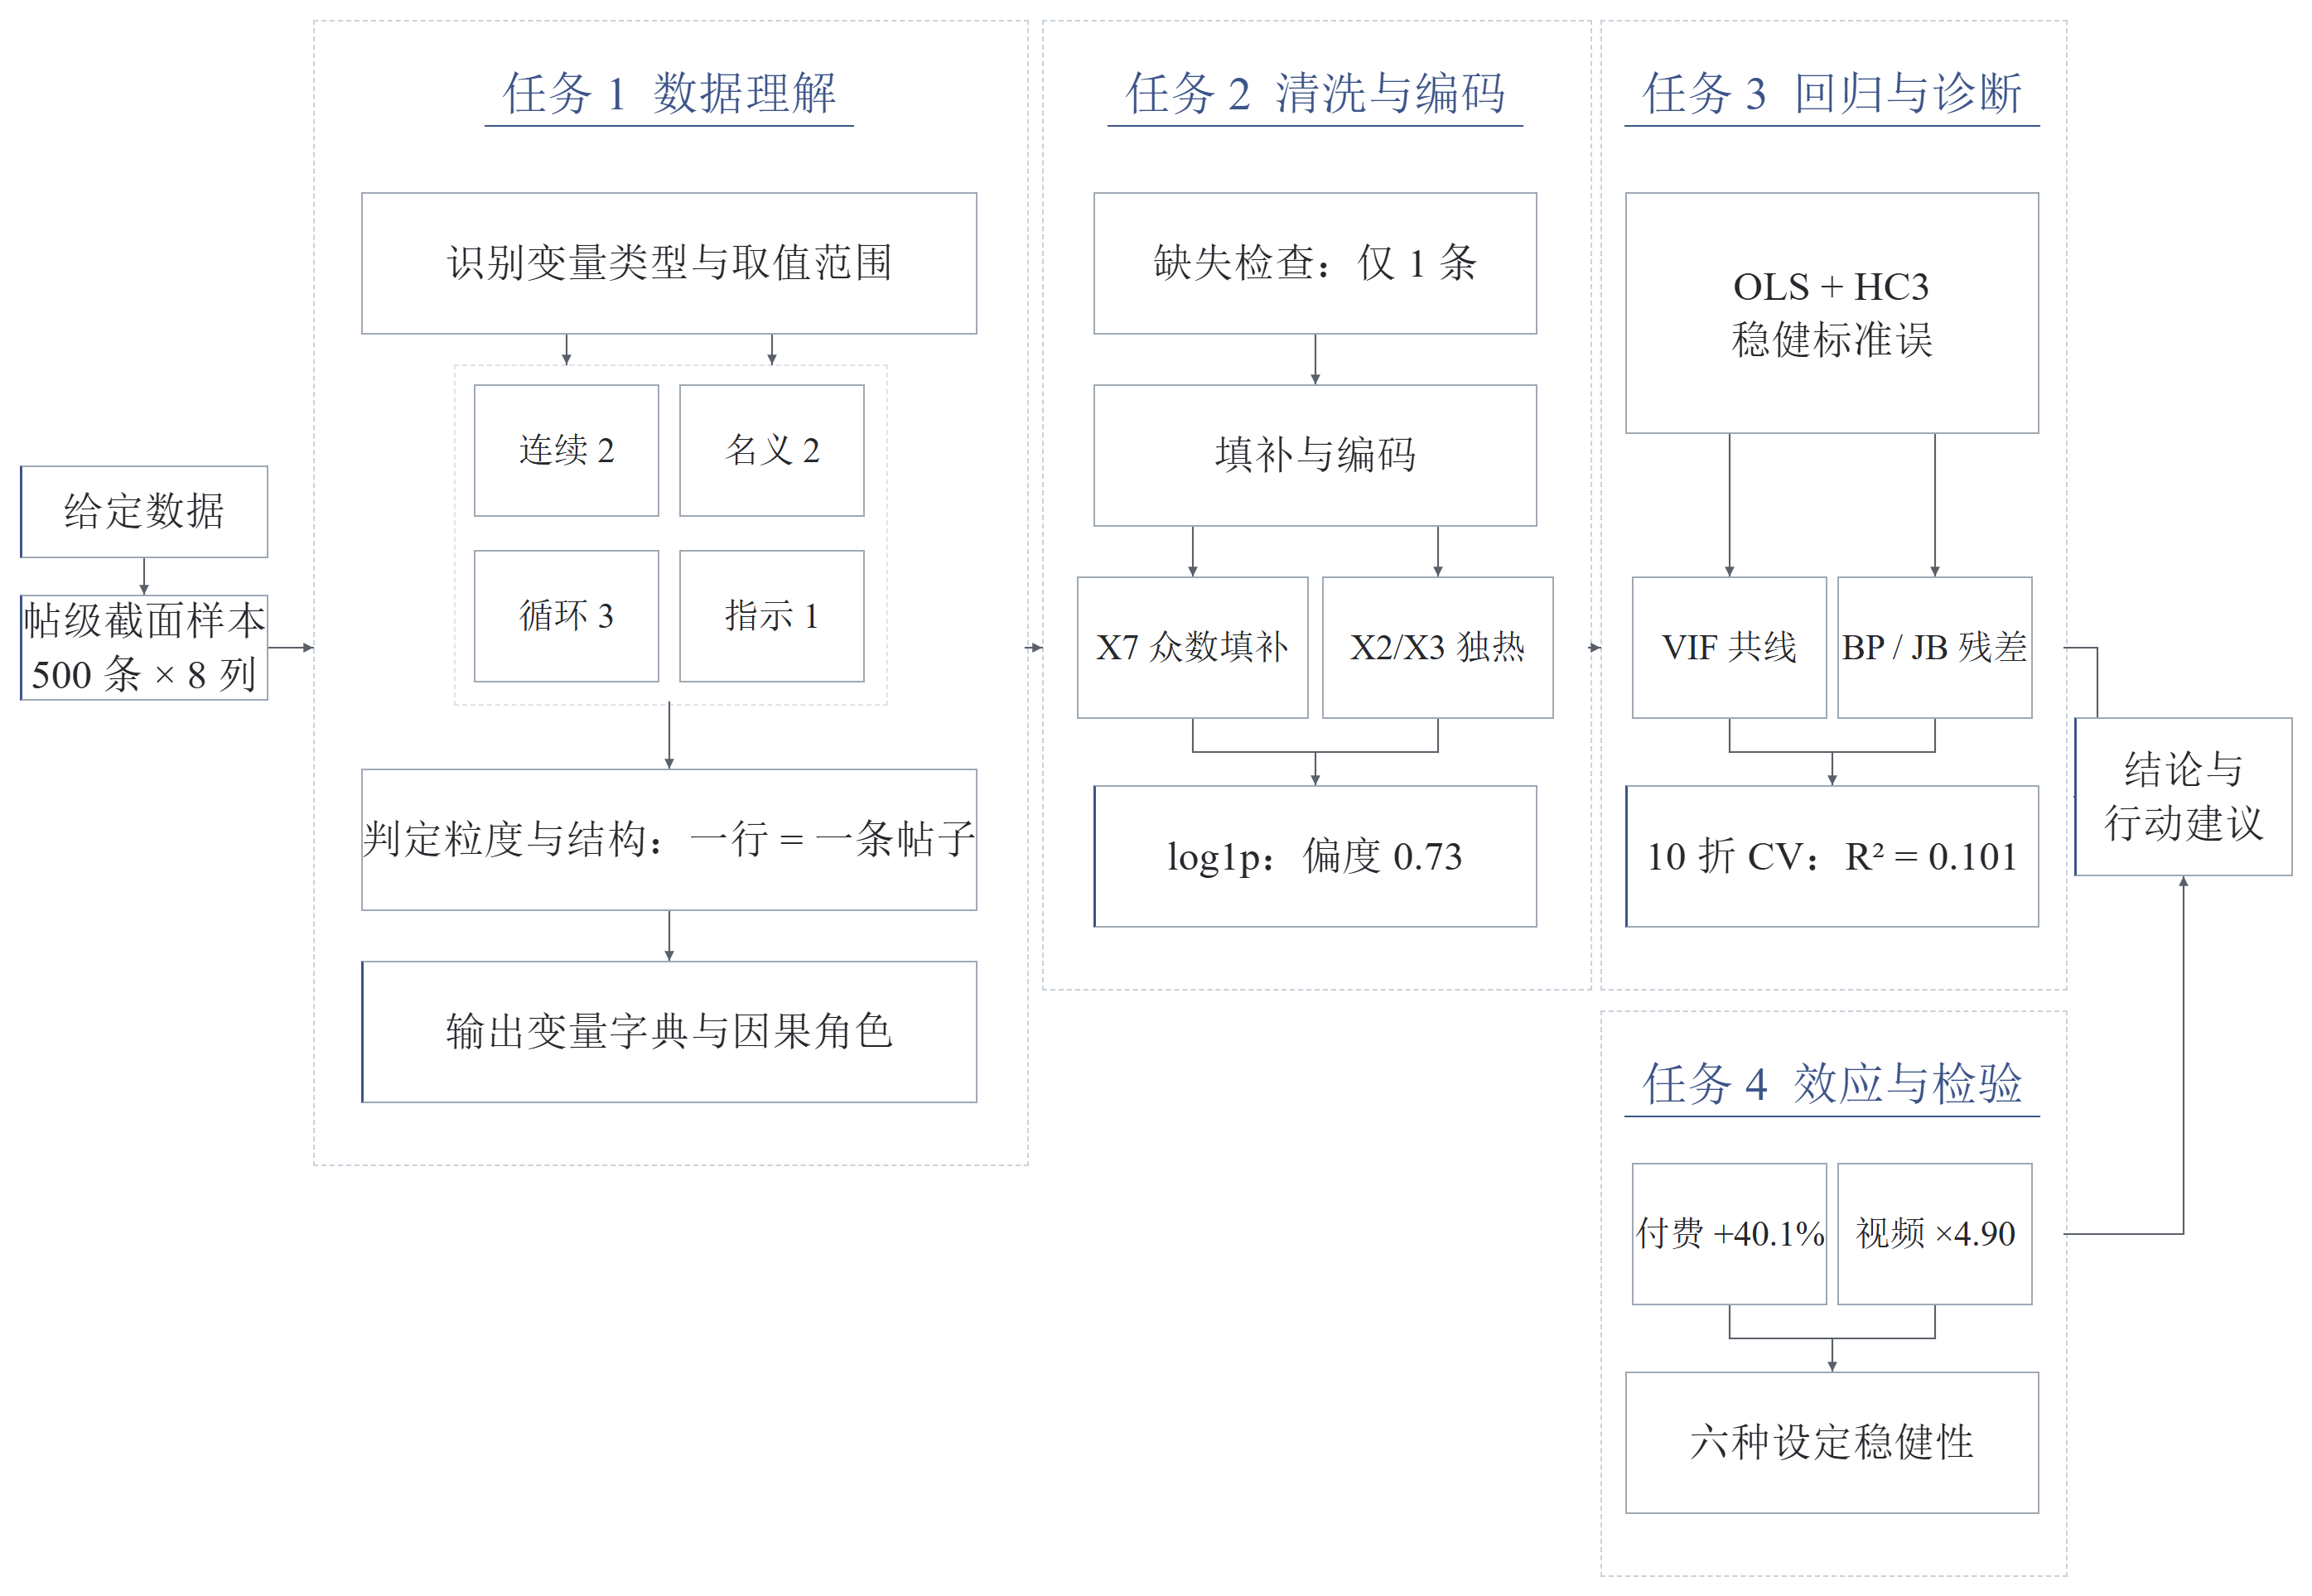
\includegraphics[width=0.86\textwidth]{../求解/临时产物/图0_技术路线.png}
  \caption{分析框架：四个任务的数据流与关键判据}
  \label{fig:route}
\end{figure}

\subsection{方法概述}

四个环节的方法与判据见表\ref{tab:method}，表中每一行都对应后文的一节，判据取可复核的阈值而不是经验描述。

\begin{table}[htbp]
  \centering
  \caption{各环节采用的方法与判别标准}
  \label{tab:method}
  {\small
  \begin{tabular}{>{\centering\arraybackslash}p{0.13\textwidth}>{\centering\arraybackslash}p{0.40\textwidth}>{\centering\arraybackslash}p{0.37\textwidth}}
    \toprule
    环节 & 采用方法 & 判别标准 \\
    \midrule
    数据诊断 & 描述统计、Pearson 与 Spearman 相关、以月份哑变量对 $\log X_1$ 的辅助回归、方差分解 & 相关系数 $|\rho|\ge0.9$、辅助回归 $R^2\ge0.9$、月内方差占比 $<5\%$，三项同时满足即判为同一变异维度 \\
    数据整理 & 众数填补、独热编码、$\log(1+Y_1)$ 与 $\log X_1$ 变换、发布时段三组合并 & 变换后偏度、峰度落入 $[-1,1]$；补缺方案差异小于标准误的 1\% \\
    回归建模 & OLS 配 HC3 稳健标准误、VIF 与条件数、Jarque--Bera / Breusch--Pagan / White / RESET / Cook 距离、十折交叉验证 & 交叉验证 $R^2$ 最大且参数个数最少；最大 VIF $<5$ \\
    效应测算 & Duan 烟雾还原、代表性画像与全样本反事实、多元正态参数模拟、Shapley 分解、六设定稳健性与子样本异质性 & 六种设定下效应方向一致、区间不跨零 \\
    \bottomrule
  \end{tabular}}
\end{table}

\subsection{主要结论}

粉丝规模与发布月份是同一条时间维度的两种写法，同时进入模型会产生不可识别的系数，模型必须以月份固定效应吸收规模趋势；控制发帖决策变量后，付费帖子的曝光比自然帖子高 40.1\%，视频帖是图片帖的 4.90 倍，主题 2 与主题 3 分别比主题 1 低 38.0\% 与 27.0\%；付费与视频效应在六种设定下方向一致、量级接近，唯一需要标注样本限制的是视频帖仅 7 条；内容主题内部的付费效应并不一致，主题 1 的付费回报明显高于主题 3。

\begin{figure}[htbp]
  \centering
  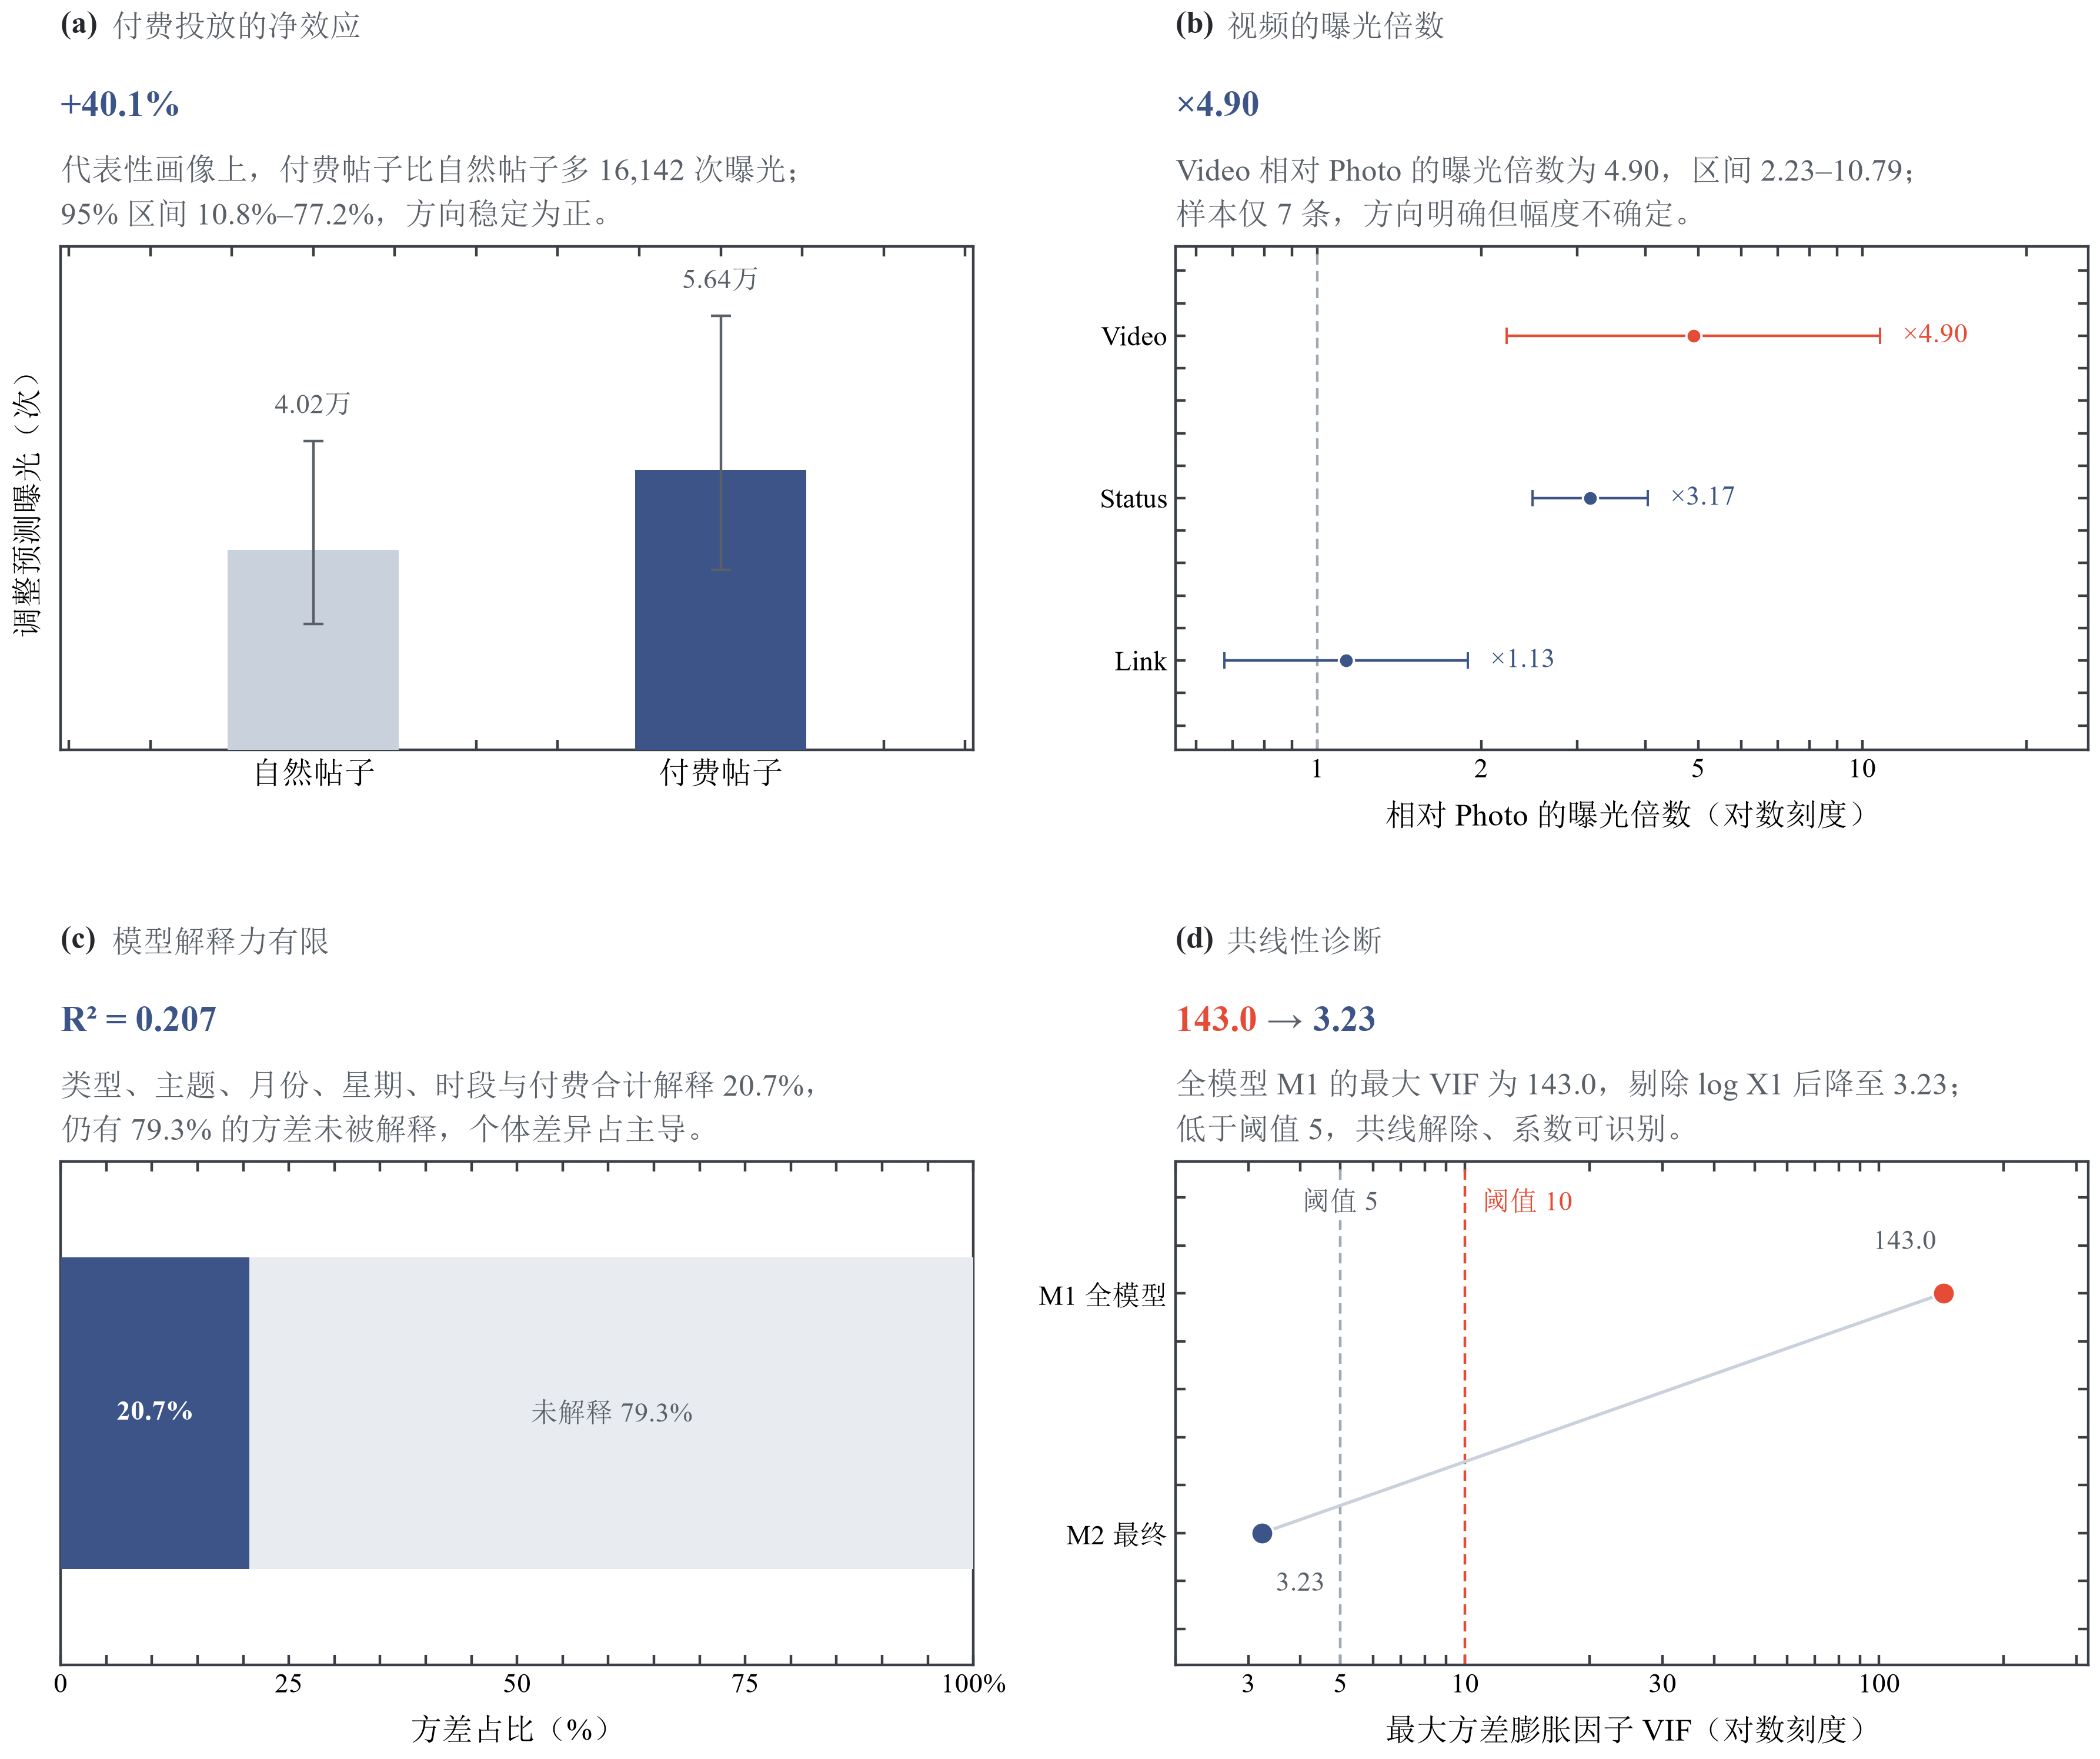
\includegraphics[width=0.72\textwidth]{../求解/临时产物/图13_核心结论总览.png}
  \caption{核心结论总览：效应、倍数、解释力与共线处理}
  \label{fig:overview}
\end{figure}
